Este capítulo describe el componente de software desarrollado para que las aplicaciones interactúen de forma autónoma con el dron. Es responsable de acceder a los sensores y actuadores del vehículo utilizando los mensajes de comunicación del protocolo MAVLink, y de traducirlos a las interfaces ICE de JdeRobot. Las aplicaciones de drones tendrán acceso a los sensores y actuadores del vehículo a través de esas interfaces.

La comunicación de nuestro driver que se comunica vía MAVLink con el dron es bidireccional. Dependiendo del módulo que se esté usando, esta comunicación puede ser dron-servidor, como por ejemplo recoger coordenadas GPS, servidor-dron, para ordenar comandos de velocidad, o bidireccional, para realizar la conexión con el servidor y envio de ACKs. 

\begin{figure}[H]
  \hspace*{-3.5cm}
  
\includegraphics[scale=0.5]{imagenes/muySencillo.png}
  \caption{Diagrama comunicación}
  \label{fig:diagramaComunicacionServerDron1}
\end{figure}


A continuación vamos a dividir en distintas fases el contenido de este driver y su ejecución:

\begin{itemize}
\item Diseño
\item Implementación
\item Operación
\end{itemize}

\section{Diseño}
\label{Diseno}
MAVLinkServer es un driver basado en el software MAVProxy y desarrollado para actuar como un \textit{middleware} de traducción. Ha sido diseñado como un controlador JdeRobot en lenguaje Python. Este driver también es responsable de mantener la comunicación, los canales abiertos y actualizados, tanto en sentido ascendente como descendente. 

En la imagen \ref{fig:diagramaHwSw} se indica como la relación entre el hardware y el software de cada componente, así como la comunicación interna o la comunicación hacia otros elementos.

\begin{figure}[H]
  \centering
  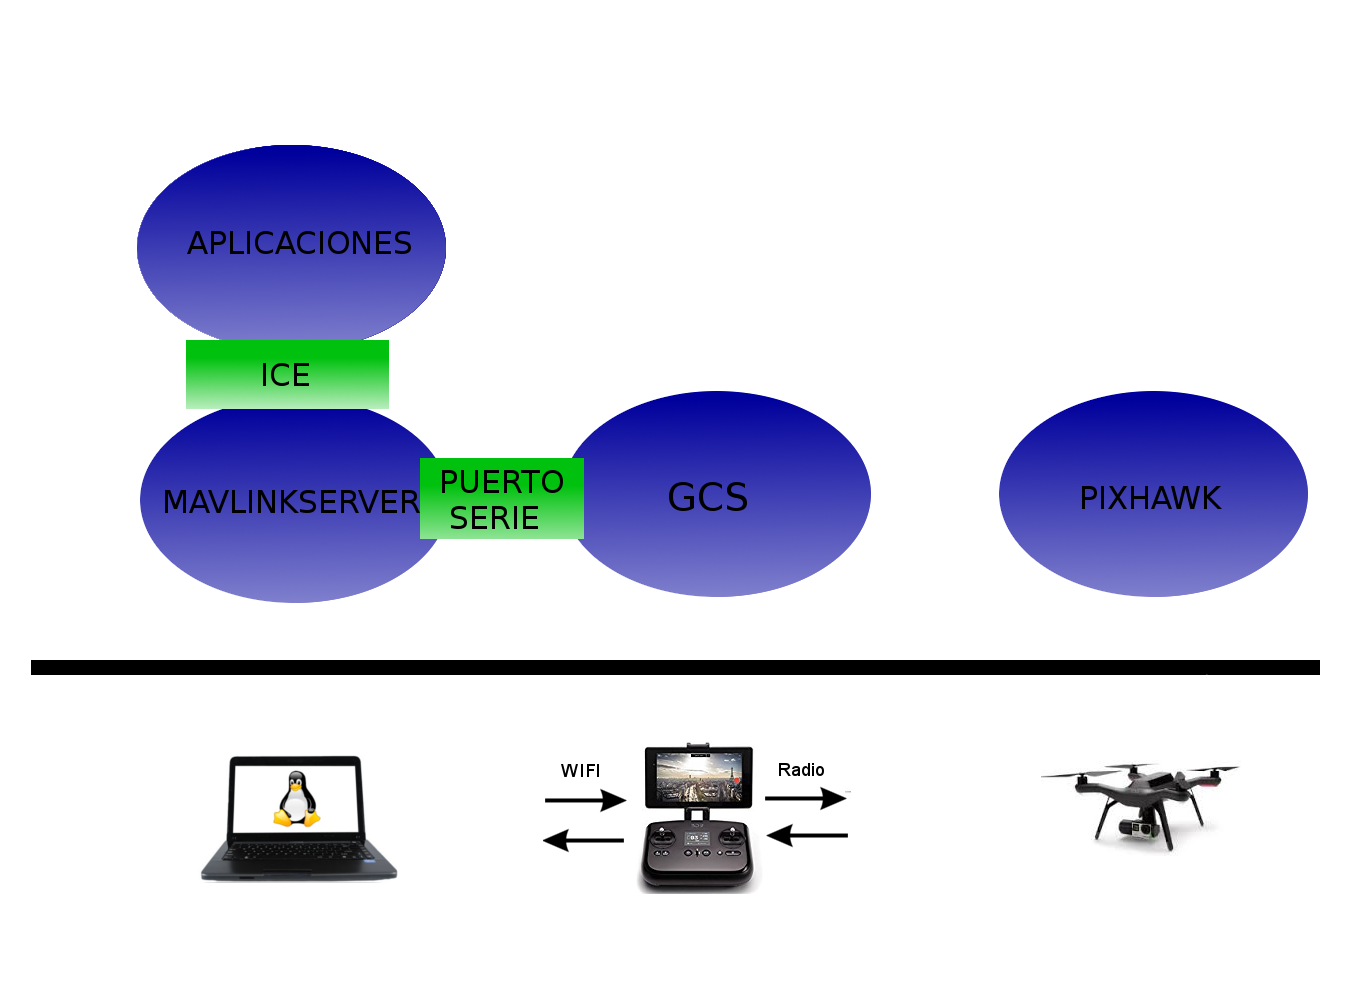
\includegraphics[scale=0.2]{imagenes/HWYSW.png}
  \caption{Diagrama de Hardware y Software}
  \label{fig:diagramaHwSw}
\end{figure}

El driver se ha diseñado combinando dos bloques: el de diálogo con el drone, usando MAVProxy, y el de dialogo con la aplicación usando interfaces ICE.

En el primer bloque, MAVLinkServer se basa en el analizador MAVProxy, la biblioteca que está a cargo de la administración de los mensajes de MAVLink. Establece la conexión con el piloto automático Pixhawk a bordo del drone, Mantiene el canal de comunicación operativo, adquiere, interpreta mensajes, crea y envía mensajes nuevos con la información solicitada u ordenada por la aplicación.

El segundo bloque, el código desarrollado está principalmente a cargo de la gestión de las interfaces JdeRobot. Es capaz de manejar la información proporcionada por el lado de MAVProxy. Regula la creación y modificación de las clases donde la información se almacena temporalmente y abre canales de comunicación ICE para hacer que el driver sea utilizable para aplicaciones JdeRobot.

Estos dos lados del driver proporcionan un controlador fiable y multi-compatible; MAVLinkServer puede conectarse con aplicaciones escritas en otros lenguajes, como C++, Python o Java, a través de las interfaces ICE de JdeRobot. La figura \ref{fig:mavLinkJdeRobotNegra} representa un esquema de entradas y salidas dentro de MAVLinkServer y sus conexiones a otras aplicaciones.


\begin{figure}[H]
  \centering
  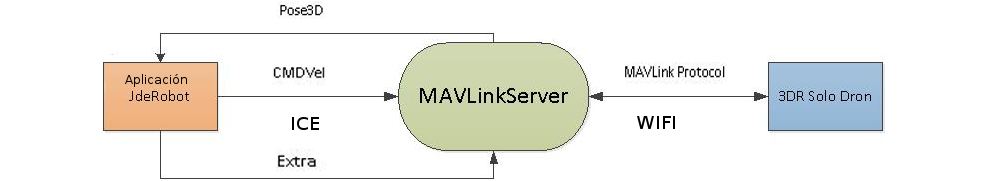
\includegraphics[scale=0.65]{imagenes/cajaNegraNueva.png}
  \caption{Diagrama de entradas y salidas bloques MAVLinkServer}
  \label{fig:mavLinkJdeRobotNegra}
\end{figure}

La información que se realiza dentro del driver se realiza a través de memoria compartida. Es necesario que la información sea bidireccional y que la memoria se este leyendo y escribiendo de la manera más ágil posible. Todas estas acciones se realizan mediante semáforos que permiten de una manera segura, en modo escritura, obtener la información de los sensores del dron e informar a la aplicación de su situación y que la aplicación envíe las acciones que debe realizar sin que ninguno de las dos acciones se vea afectada por la otra.

\begin{figure}[H]
  \centering
  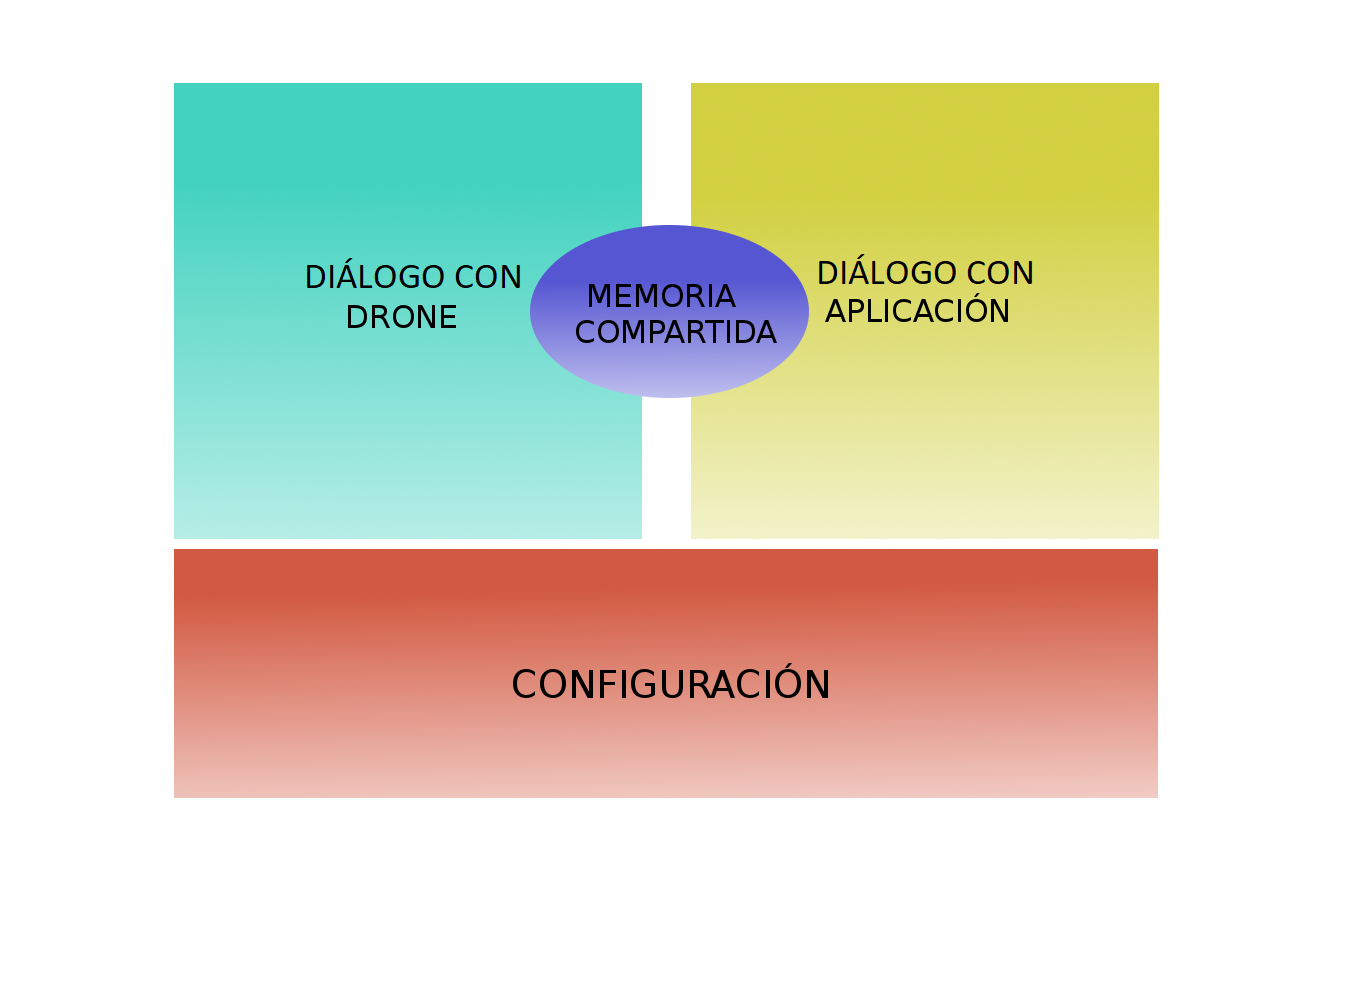
\includegraphics[scale=0.2]{imagenes/MEMORIACOMPARTIDA.png}
  \caption{Diagrama de memoria en MAVLinkServer}
  \label{fig:memoriaCompartida}
\end{figure}

Las interfaces JdeRobot utilizadas en este proyecto son Pose3D (proporciona la posición y medidas del vehículo), CMDVel (para enviar los comandos de velocidad) y Extra (para despegue y aterrizaje). Pose3D hace uso de cuaterniones en lugar de ángulos de Euler. Esto se hace para evitar singularidades angulares y superposiciones, y computacionalmente son más simples que otros formalismos de posicion como ángulos de Euler o una matriz de coseno de dirección.


\section{Configuración}

En este apartado vamos a explicar todos los pasos a seguir para realizar una configuración, que nos puede ofrecer dependiendo de este tipo de configuración y todas las librerías que tenemos a nuestra disposición.

Antes de que el driver pueda ejecutar correctamente hay que configurar el software MAVProxy del sistema.


\subsection{Configuración de MAVProxy}
\label{Pre-Configuracion}


Para llevar a cabo esta configuración de MAVProxy debemos tener en cuenta la existencia de una serie de ficheros, llamados módulos, que cada uno de ellos nos va a facilitar una utilidad diferente, que pueden ir desde conocer la batería, altura del dron o configurar una web-cam.

Estos módulos se pueden descargar desde el repositorio oficial de MAVLink o crear una librería propia e implementarla. En el siguiente código que se muestra se puede ver como esta implementa obtener la información de la batería a través del voltaje que desprende:
\footnote{\url{https://github.com/ArduPilot/MAVProxy}}.

\begin{lstlisting}[frame=single]
    def vcell_to_battery_percent(self, vcell):
        '''convert a cell voltage to an approximate
        percentage battery level for a LiPO'''
        if vcell > 4.1:
            # above 4.1 is 100% battery
            return 100.0
        elif vcell > 3.81:
            # 3.81 is 17% remaining, from flight logs
            return 17.0 + 83.0 * (vcell - 3.81) / (4.1 - 3.81)
        elif vcell > 3.2:
            # below 3.2 it degrades fast. It's dead at 3.2
            return 0.0 + 17.0 * (vcell - 3.20) / (3.81 - 3.20)
        # it's dead or disconnected
        return 0.0
\end{lstlisting}

\subsection{Configuración del driver MAVLinkServer}

El fichero de configuración que usa el servidor únicamente se limita a establecer los puertos mediante los cuales se va a realizar la comunicación de cara a un usuario.


\begin{lstlisting}[frame=single]
Camera:
  Server: 1 # 0 -> Deactivate, 1 -> Ice , 2 -> ROS
  Proxy: "default -h 0.0.0.0 -p 9999"
  Format: RGB8
  Topic: "/MavLink/image_raw"
  Name: MavLinkCamera

Pose3D:
  Server: 1 # 0 -> Deactivate, 1 -> Ice , 2 -> ROS
  Proxy: "default -h 0.0.0.0 -p 9998"
  Topic: "/MavLink/Pose3D"
  Name: MavLinkPose3d

CMDVel:
  Server: 1 # 0 -> Deactivate, 1 -> Ice , 2 -> ROS
  Proxy: "default -h 0.0.0.0 -p 9997"
  Topic: "/MavLink/CMDVel"
  Name: MavLinkCMDVel

Navdata:
  Server: 1 # 0 -> Deactivate, 1 -> Ice , 2 -> ROS
  Proxy: "default -h 0.0.0.0 -p 9996"
  Topic: "/MavLink/Navdata"
  Name: MavLinkNavdata

Extra:
  Server: 1 # 0 -> Deactivate, 1 -> Ice , 2 -> ROS
  Proxy: "default -h 0.0.0.0 -p 9995"
  Topic: "/MavLink/Extra"
  Name: MavLinkExtra
\end{lstlisting}



\subsection{Script de arranque}
\label{Script de arranque}

El script de arranque se encargara de ejecutar todos los comandos previos y el servidor. El script se encuentra en MAVProxy/MAVProxyWinLAN.sh, deberemos averiguar la IP que levanta el dron, en nuestro caso, con el 3DR Solo, dicha IP la levanta el mando como hemos comentado en la introducción de este capitulo. Deberemos modificar el script con la IP del dron a la que nos hayamos conectado y ejecutarlo sin parámetros adicionales. 

Se necesita tener preinstalado tanto pyserial como una versión de pyvmavlink superior a la 1.1.50. Se realiza una descarga de todos los módulos, construye un directorio llamado MavProxy.egg en /home/USER/.local/python3.5/site-packages con el fin de tener almacenados todos los paquetes necesarios y con permisos suficientes. 

La configuración que se puede modificar a nivel de script está relacionada con el tipo de conexión que se quiere mantener con el dron. Esta conexión tiene valores por defecto pero se puede modificar si así se desea. Los comandos que se muestran en la tabla son un ejemplo de la versatilidad que tiene el servidor. A través de estos paquetes generados es posible acceder a los comandos que nos proporciona MAVLink. A continuación se proporciona un listado de los posibles comandos opcionales que se pueden añadir al script de arranque y una breve explicación de cada uno de ellos se realiza a continuación:

\begin{center}
  \label{scriptArranqueComandos}
  \begin{tabular}{ | l | p{8cm} | p{5cm} |}
    \hline
    Comando & Acción & Valor por defecto \\ \hline
    master & Puerto maestro MAVLink y baudrate opcional &  \\ \hline
    udp & Arranca el servidor udp & TCP \\ \hline
    tcp & Arranca el servidor tcp & TCP \\ \hline
    out & Puerto de salida MAVLink & \\ \hline
    baudrate & & 57600  \\ \hline
    sitl& Puerto de salida, esta opción únicamente es necesaria en caso de no tener disponible un dron.& \\ \hline
    streamratedest &  MAVLink stream rate & 4 \\ \hline
    source-system & Código fuente MAVLink & 255 \\ \hline
    source-component & Componente origen MAVLink & 0 \\ \hline
    target-system & Sistema destino MAVLink & 0  \\ \hline
    target-component & Componente destino MAVLink & 0 \\ \hline
    logfile & Fichero de logs & mav.tlog \\ \hline
    append-log & Añadir al fichero de log ya existente & False  \\ \hline
    continue & Continua el log& False \\ \hline
    quadcopter& Usar acciones de control para cuadricopteros&  False\\ \hline
    setup& Arrancar en modo setup & False \\ \hline
    nodtr& Deshabilitar DTR(Data Terminal Ready) & False \\ \hline
    show-errors& Mostrar errores MAVLink& False \\ \hline
    speech& Usar texto para hablar & False \\ \hline
    aircraft& Establecer nombre para el dron (Visual en mensajes)& None \\ \hline
    cmd& Comandos a ejecutar tras el arranque & None  \\ \hline
    console& Usar consola GUI para introducir comandos &  \\ \hline
    map& Carga un mapa de la zona&  \\ \hline
    load-module& Carga un modulo especifico, puede ser utilizado tantas veces como sea necesario separando con ",")&  \\ \hline
    mav09& Usa protocolo MAVLink 0.9 & False \\ \hline
    auto-protocol&Auto detecta versión de protocolo MAVLink& False \\ \hline
  \end{tabular}
\end{center}
\begin{center}
  \label{scriptArranqueComandos2}
  \begin{tabular}{ | l | p{8cm} | p{5cm} |}
  \hline
    Comando & Acción & Valor por defecto \\ \hline
    nowait&No realiza comunicación continua con el dron (HearthBeat) &  False\\ \hline
    dialect & Dialecto MAVLink& ardupilotmega \\ \hline
    rtscts& Habilita control de comunicación vía RTS/CTS&  False\\ \hline
    mission& Nombre de la misión& None \\ \hline
    daemon & Arranca en modo daemon, no muestra shell interactiva & False \\ \hline
    profile& Arranca el Yappi python profiler& False \\ \hline
    state-basedir& Directorio base para logs& None \\ \hline
    version& Muestra información sobre la versión& False \\ \hline
    default-modules& Módulos por defecto al iniciar.& log, wp, rally, fence, param, relay, tuneopt, arm, mode, calibration, rc, auxopt, misc, cmdlong, battery, terrain, output \\ \hline
    \hline
  \end{tabular}
\end{center}

Los comandos que se muestran en la tabla \ref{comandos}, sólo se pueden ejecutar si en el paso anterior se ha introducido el comando "--console", de cualquier otra manera, no se muestra la consola mediante la cual se pueden introducir comandos. Estos comandos tienen una labor de modificar la experiencia de vuelo del dron o muestra los valores que nos pueden proporcionar sus sensores:

\begin{center}
  \label{comandos}
  \begin{tabular}{ | l | p{10cm} |}
  \hline
  Comando & Acción \\ \hline
  reboot& Reinicia el dron\\ \hline
  arm & Habilita los medidores propios del dron. Ejemplo de ejecución: check (all |baro|compass|gps|ins|params |rc|voltage|battery),uncheck (all|baro|compass |gps|ins|params|rc| voltage|battery), list,throttle,safetyon,safetyoff (arm throttle arranca hélices del dron)\\ \hline
  disarm& Detiene los motores del dron \\ \hline
  takeoff& Despegue del dron\\ \hline
  land&Aterrizaje del dron \\ \hline
  mode& Cambia el modo de vuelo\\ \hline
  velocity& Establece una velocidad en los ejes x,y,z\\ \hline
  parachute& Habilita un aterrizaje del dron si pierde conexión o la batería es baja. Ejemplo de ejecución: parachute [enable|disable|release]\\ \hline
  bat& Muestra batería del dron\\ \hline
  alt& Muestra altitud del dron\\ \hline
    \hline
  \end{tabular}
\end{center}
\section{Diálogo con las aplicaciones}


MAVLinkServer lanza varios hilos para canales de comunicación ICE, uno para cada tipo de información. A pesar de que solo Pose3D, CMDVel y Extra deben ser realmente utilizados, el driver ofrece las interfaces restantes para compatibilidad y usos futuros. Dichos hilos de comunicación realizan operaciones de lectura y escritura en memoria necesarias para la comunicación entre los distintos componentes ICE o comunicación entre el puerto serie y los comandos que se le proporcionan al dron.

Cada subproceso hace uso de su propia función donde se realiza la configuración de ICE.
Allí se realiza la publicación de ICE y es importante garantizar qué datos se envían, para que otras aplicaciones obtengan la información correctamente y garanticen la compatibilidad.
El mismo procedimiento se realiza para todas las interfaces.

El primer paso es definir las interfaces ICE correspondientes. MAVLinkServer suministra todas las interfaces JdeRobot para el acceso de drones desde cualquier componente externo. Aquí está un ejemplo de la interfaz Pose3D.

\begin{lstlisting}[frame=single]
import jderobot, time, threading

lock = threading.Lock()

class Pose3DI(jderobot.Pose3D):

    def __init__(self,_x,_y,_z,_h,_q0,_q1,_q2,_q3):

        self.x = _x
        self.y = _y
        self.z = _z
        self.h = _h
        self.q0 = _q0
        self.q1 = _q1
        self.q2 = _q2
        self.q3 = _q3

        print ("Pose3D start")

    def setPose3DData(self, data, current=None):

        lock.acquire()

        self.x = data.x
        self.y = data.y
        self.z = data.z
        self.h = data.h
        self.q0 = data.q0
        self.q1 = data.q1
        self.q2 = data.q2
        self.q3 = data.q3

        lock.release()

        return 0

    def getPose3DData(self, current=None):

        time.sleep(0.05) # 20Hz (50ms) rate to tx Pose3D

        lock.acquire()

        data = jderobot.Pose3DData()
        data.x = self.x
        data.y = self.y
        data.z = self.z
        data.h = self.h
        data.q0 = self.q0
        data.q1 = self.q1
        data.q2 = self.q2
        data.q3 = self.q3

        lock.release()

        return data
\end{lstlisting}  

Esta clase hereda "jderobot.Pose3D" y se definen las funciones correspondientes. Eso
se puede notar el uso de "bloqueos" de programación para proteger los datos almacenados en la clase. Esto se debe a que MAVLinkServer actualiza constantemente la información provista por los sensores y también la publica constantemente a través de ICE. Esto podría causar condiciones de carrera. Con el uso de los bloqueos en las clases, la información no se podía leer mientras otra tarea estaba escribiendo en ella y viceversa, asegurando la administración correcta de la información en exclusión mutua.

\begin{figure}[H]
  \centering
  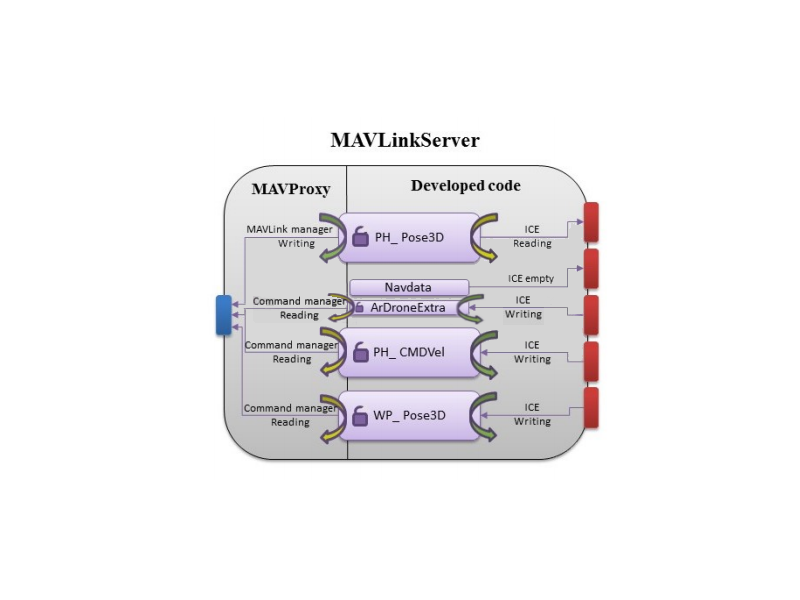
\includegraphics[scale=0.6]{imagenes/MavProxyPorDentro.png}
  \caption{Gestión de memoria}
  \label{fig:MavProxyInside}
\end{figure}

La interfaz CMDVel y Extra tiene la misma estructura que Pose3D, también con el uso de cierres.

\begin{lstlisting}[frame=single]

import jderobot, time, threading

lock = threading.Lock()

class CMDVelI(jderobot.CMDVel):

    def __init__(self,lx,ly,lz,ax,ay,az):

        self.linearX = lx
        self.linearY = ly
        self.linearZ = lz
        self.angularX = ax
        self.angularY = ay
        self.angularZ = az

        #print ("cmdvel start")

    #def __del__(self):

        #print ("cmdvel end")


    def setCMDVelData(self, data, current=None):

        lock.acquire()

        self.linearX = data.linearX
        self.linearY = data.linearY
        self.linearZ = data.linearZ
        self.angularX = data.angularX
        self.angularY = data.angularY
        self.angularZ = data.angularZ

        lock.release()

        return 0

    def getCMDVelData(self, current=None):

        time.sleep(0.05)  # 20Hz (50ms) rate to rx CMDVel

        lock.acquire()

        data = jderobot.CMDVelData()
        data.linearX = self.linearX
        data.linearY = self.linearY
        data.linearZ = self.linearZ
        data.angularX = self.angularX
        data.angularY = self.angularY
        data.angularZ = self.angularZ
        lock.release()

        return data
        
\end{lstlisting} 

\begin{lstlisting}[frame=single]
import jderobot, time, threading

lockLand = threading.Lock()
lockTakeOff = threading.Lock()

class ExtraI(jderobot.ArDroneExtra):

    def __init__(self):

        print ("Extra start")
        self.landDecision = False
        self.takeOffDecision = False

    def land(self,xxx):
        self.setLand(True)
        lockLand.acquire()
        landDecision = self.landDecision
        lockLand.release()

        return landDecision

    def takeoff(self,xxx):
        self.setTakeOff(True)
        lockTakeOff.acquire()
        takeOffDecision = self.takeOffDecision
        lockTakeOff.release()

        return takeOffDecision

    def setLand(self,decision):
        lockLand.acquire()
        self.landDecision = decision
        lockLand.release()

    def setTakeOff(self, decision):
        lockTakeOff.acquire()
        self.takeOffDecision = decision
        lockTakeOff.release()

    def setExtraData(self, data, current=None):

        lockLand.acquire()
        self.landDecision = data.landDecision
        lockLand.release()

        lockTakeOff.acquire()
        self.takeOffDecision = data.takeOffDecision
        lockTakeOff.release()

        return 0

\end{lstlisting}  

\section{Diálogo directo con el drone}

Por otro lado solo tiene una conexión con el puerto de comunicación con el dron (puerto serie). La gestión de estos 3 hilos de comunicación, respecto al único puerto serie que se mantiene por parte del dron, se basa en prioridades. Extra es el más prioritario al ser la parte más restrictivo, este componente predomina sobre los otros 2 debido a la importancia de las órdenes que envía. Pose3D recibe la información del dron para actualizar la posición en un canal únicamente de lectura del puerto serie. Por otro lado, conviven al mismo tiempo tanto CMDVel como Pose3D a la hora de realizar enviar comandos de velocidad y/o posición.

\begin{lstlisting}[frame=single]
	mpstate.status.thread = threading.Thread(target=main_loop, 
    						name='main_loop')
    mpstate.status.thread.daemon = True
    mpstate.status.thread.start()

    #Open an ICE TX communication and leave it open in a parallel thread

    PoseTheading = threading.Thread(target=openPose3DChannel, 
    				args=(PH_Pose3D,), name='Pose_Theading')
    PoseTheading.daemon = True
    PoseTheading.start()

    # Open an ICE RX communication and leave it open in a parallel thread

    CMDVelTheading = threading.Thread(target=openCMDVelChannel, 
    				args=(PH_CMDVel,), name='CMDVel_Theading')
    CMDVelTheading.daemon = True
    CMDVelTheading.start()

    # Open an ICE TX communication and leave it open in a parallel thread

    CMDVelTheading = threading.Thread(target=openExtraChannel, 
    				args=(PH_Extra,), name='Extra_Theading')
    CMDVelTheading.daemon = True
    CMDVelTheading.start()

    # Open an ICE channel empty

    CMDVelTheading = threading.Thread(target=openNavdataChannel, 
    					args=(), name='Navdata_Theading')
    CMDVelTheading.daemon = True
    CMDVelTheading.start()

    # Open an ICE TX communication and leave it open in a parallel thread

    PoseTheading = threading.Thread(target=openPose3DChannelWP, 
    				args=(WP_Pose3D,), 
                    name='WayPoint_Theading')
    PoseTheading.daemon = True
    PoseTheading.start()

 # Open an MAVLink TX communication and leave it open in a parallel 
    # thread
    #
    PoseTheading = threading.Thread(target=sendCMDVel2Vehicle, 
    				args=(PH_CMDVel,PH_Pose3D,), 
                    name='TxCMDVel_Theading')
    PoseTheading.daemon = True
    PoseTheading.start()


    # Open an MAVLink TX communication and leave it open in a parallel thread

    PoseTheading = threading.Thread(target=sendWayPoint2Vehicle,
    				args=(WP_Pose3D,), 
                    name='WayPoint2Vehicle_Theading')
    PoseTheading.daemon = True
    PoseTheading.start()

    # Open an MAVLink TX communication and leave it open in a parallel thread

    PoseTheading = threading.Thread(target=landDecision, 
    				args=(PH_Extra,), 
                    name='LandDecision2Vehicle_Theading')
    PoseTheading.daemon = True
    PoseTheading.start()
   
\end{lstlisting}

MAVproxy está constantemente manejando los mensajes MAVLink en un hilo paralelo en un bucle infinito. Este módulo lo aprovecha y refresca la información del sensor necesario. Como un controlador de alto nivel, este programa no interfiere con la fusión de datos realizado por Pixhawk y confía en su rendimiento, cuya fiabilidad ha sido ampliamente probado.

\begin{figure}[H]
  \centering
  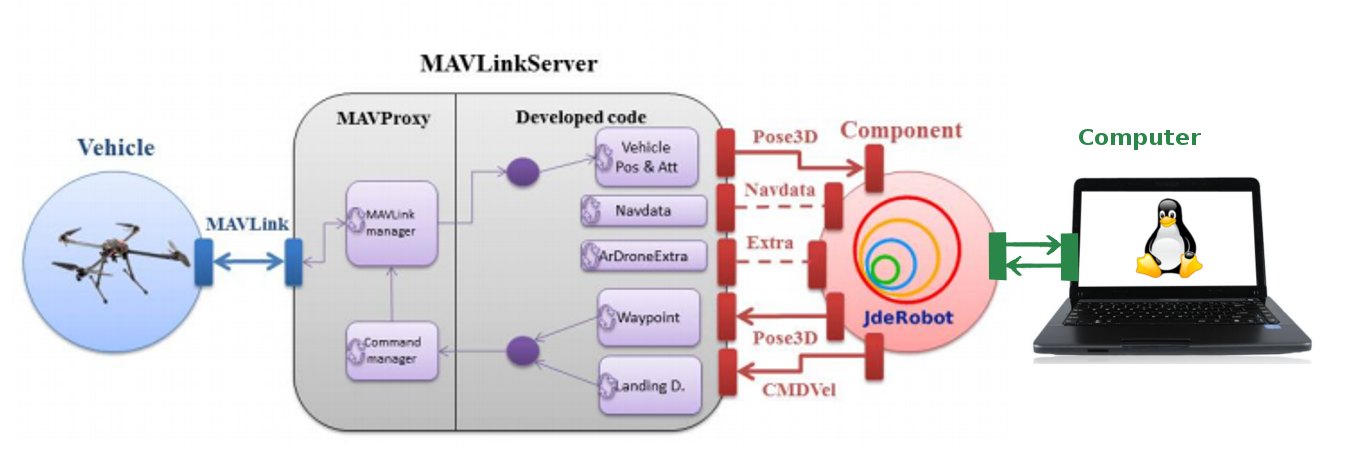
\includegraphics[scale=0.35]{imagenes/cajaTrasparente.png}
  \caption{Diagrama bloques MAVLink-JdeRobot con detalle}
  \label{fig:mavLinkJdeRobotTrasparente}
\end{figure}


Para llevar a cabo esta carga el primer paquete que se carga es "Link", este paquete se encarga de la conexión entre el servidor y el dron. Es necesario conocer la dirección IP que levanta este dron, que ya habremos configurado en el paso \ref{Script de arranque}. Tras lograr la conexión se establece un periodo de "checkeo" necesario para no perder la conexión con el dron en caso de llegar a una distancia límite o un fallo de conexión, en cuyo caso se procede a detenerse el dron. Esto se debe a periódicamente se debe realizar una comunicación entre el dron y el servidor, aunque no se llegue a mandar ningún comando, ya sea de velocidad o algún tipo de acción, el servidor por su parte comunicara que aun esta conectado. Después de un tiempo sin conexión, aproximadamente unos 10-15 segundos, el dron procederá a realizar un despegue. 



\begin{lstlisting}[frame=single]
def periodic_tasks():
    '''run periodic checks'''
    if mpstate.status.setup_mode:
        return

    if (mpstate.settings.compdebug & 2) != 0:
        return

    if mpstate.settings.heartbeat != 0:
        heartbeat_period.frequency = mpstate.settings.heartbeat

    if heartbeat_period.trigger() and mpstate.settings.heartbeat != 0:
        mpstate.status.counters['MasterOut'] += 1
        for master in mpstate.mav_master:
            send_heartbeat(master)

    if heartbeat_check_period.trigger():
        check_link_status()

    set_stream_rates()

    for (m,pm) in mpstate.modules:
        if hasattr(m, 'idle_task'):
            try:
                m.idle_task()
            except Exception as msg:
                if mpstate.settings.moddebug == 1:
                    print(msg)
                elif mpstate.settings.moddebug > 1:
                    exc_type, exc_value, exc_traceback = sys.exc_info()
                    traceback.print_exception(exc_type, exc_value, 
                    		exc_traceback,limit=2, file=sys.stdout)

        # also see if the module should be unloaded:
        if m.needs_unloading:
            unload_module(m.name)
\end{lstlisting}
            
Al acabar toda la carga de los módulos establecemos la conexión con los puertos necesarios con JdeRobot para poder pilotar el dron. Los módulos que usamos son Pose3D, CMDVel y Extra. Para cada uno de ellos vamos a necesitar crear 1 threads, para recibir los comandos que nos deseen enviar por el canal. Cada módulo lo necesitaremos por los siguientes motivos:

\begin{lstlisting}[frame=single]

def load_module(modname, quiet=False):
    '''load a module'''
    modpaths = ['MAVProxy.modules.mavproxy_%s' % modname, modname]
    for (m,pm) in mpstate.modules:
        if m.name == modname:
            if not quiet:
                print("module %s already loaded" % modname)
            return False
    for modpath in modpaths:
        try:
            m = import_package(modpath)
            imp.reload(m)
            module = m.init(mpstate)
            if isinstance(module, mp_module.MPModule):
                mpstate.modules.append((module, m))
                if not quiet:
                    print("Loaded module %s" % (modname,))
                return True
            else:
                ex = "%s.init did not return a MPModule instance" % modname
                break
        except ImportError as msg:
            ex = msg
            if mpstate.settings.moddebug > 1:
                import traceback
                print(traceback.format_exc())
    print("Failed to load module: %s. Use 'set moddebug 3' in the MAVProxy console to enable traceback" % ex)
    return False
\end{lstlisting}

\begin{itemize}
\item CMDVel: Este módulo nos dará lo necesario para poder mover el dron en los ejes x,y,z y sobre el yaw. La velocidad máxima que se le puede dar al dron a través del interfaz ICE en cada dirección viene dado en una escala de 0 a 1.  
\begin{lstlisting}[frame=single]
def sendCMDVel2Vehicle(CMDVel,Pose3D):
    absolute = 0
    relative = 1

    while True:

        CMDVel2send = CMDVel.getCMDVelData()
        Pose3D2send = Pose3D.getPose3DData()
        #print(Pose3D2send)
        NEDvel = body2NED(CMDVel2send, Pose3D2send) # [x,y,z]
        linearXstring = str(NEDvel[0])
        linearYstring = str(NEDvel[1])
        linearZstring = str(NEDvel[2])

        #CMDVel.angularZ -1 y 1

        angular = CMDVel.angularZ

        if angular >= 0:
            direction = str(1)
        else:
            angular = -angular
            direction = str(-1)

        angularZstring = str(angular*30)

        movement = str(relative)

        velocitystring = 'velocity '+ linearXstring + ' ' + 
        				  linearYstring + ' ' + 
                          linearZstring
        angularString = 'setyaw ' + angularZstring + ' ' + 
        				  direction + ' ' + movement

        process_stdin(velocitystring) 
        process_stdin(angularString)
\end{lstlisting}
\item Extra: Este módulo nos dará la facilidad de despegar y de aterrizar. Debido al protocolo MAVLink, el sistema de despegue se compone en 3 estados, que agruparemso bajo la misma orden ICE de despegue. Durante la fase de despegue el dron no admite ningún comando a excepción del comando "land" para aterrizar, o en caso del despegue, para detener el despegue.  Este despegue dura aproximadamente unos 10 segundos hasta que se estabiliza en el aire por motivos de seguridad. \begin{enumerate}
						\item El arranque de las hélices. 
                        \item Despegue del dron.
                        \item Habilitar comandos de velocidad.
						\end{enumerate}
\item Pose3d: Este módulo nos indicará la posición del dron en todo momento, así como su orientación y altitud. Esta conexión nos va a servir tanto a la hora de aterrizar y despegar usando el otro módulo comentado Extra, para saber si puede aterrizar en un determinado momento o debe disminuir su altura antes de parar los motores.

\end{itemize}


